\section{Support Vector Machines}

\subsection{Characteristics}
\begin{itemize}
    \item Supervised learning algorithm usually used for classification
    \item Binary classifier, so it is not probabilistic
    \item Linear classifier, but can perform nonlinear classification using particular kernels;
    \item Use regularized logistic regression
\end{itemize}

\subsection{Relation between Logistic Regression and SVM}
Logistic classification has the following formula:

\begin{equation} \tag*{}
    h_\theta(x) = g(\theta^Tx) = \cfrac{1}{1+e^{\theta^Tx}}
\end{equation}
Where:
\begin{equation} \tag*{}
    g(z) = \cfrac{1}{1+e^{-z}}
\end{equation}
The cost function for logistic regression given an example $i$ and a vector of weights $\theta$ is as follows:
\begin{equation} \tag*{}
    \text{cost} = -y^i \cdot \log(\frac{1}{1+e^{\theta^Tx^i}}) - (1-y^i) \cdot \log(1-\frac{1}{1+e^{\theta^Tx^i}})
\end{equation}
What we'd like logistic regression to do:
\begin{itemize}
    \item if $y = 1$, we want $h_\theta(x) \approx 1, \theta^Tx \gg 0$
    \item if $y = 0$, we want $h_\theta(x) \approx 0, \theta^Tx \ll 0$
\end{itemize}
\begin{center}
    \begin{tabular}{c}
        \\ 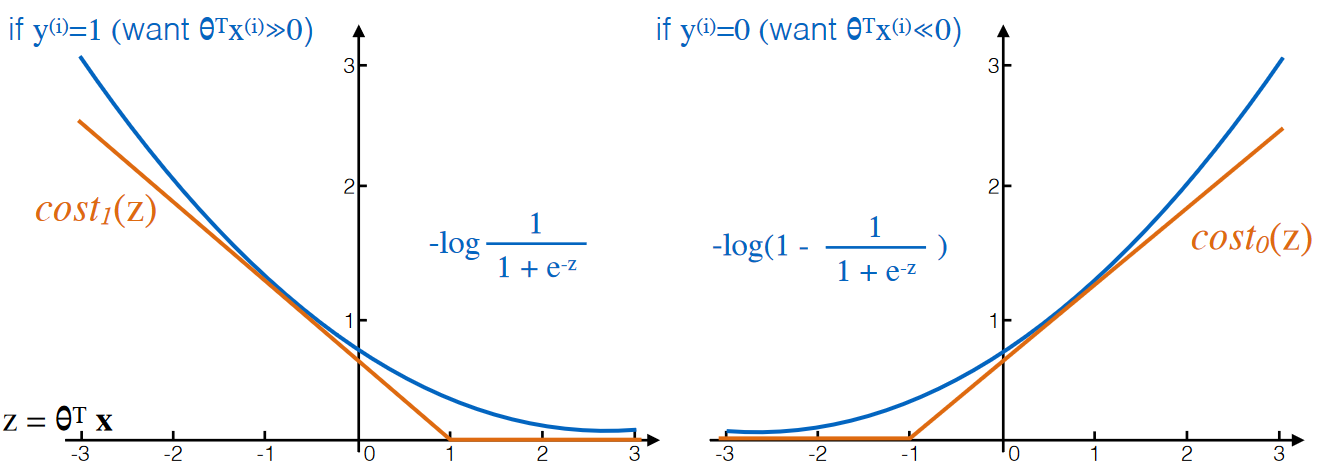
\includegraphics[width=0.9\textwidth]{images/SVM1.png} \\ \\
    \end{tabular}
\end{center}
The objective function of an SVM can be written as follows:
\begin{equation} \tag*{}
    \min \frac{1}{\lambda} \sum^m_{i=1} [y^i \cdot \text{cost}_1(\theta^Tx^i) + (1 - y^i) \cdot \text{cost}_0(\theta^Tx^i)] + \frac{1}{2} \sum^n_{j=i}\theta^2_j
\end{equation}
The functions cost$_1$ and cost$_0$ allow us to create a decision boundary.

\newpage
\subsection{Decision Boundary}
The decision boundary allows too ambiguous results to be penalized, for example with a decision boundary between $1$ and $-1$ values of $\theta^Tx$ will be penalized.
\begin{center}
    \begin{tabular}{c}
        \\ 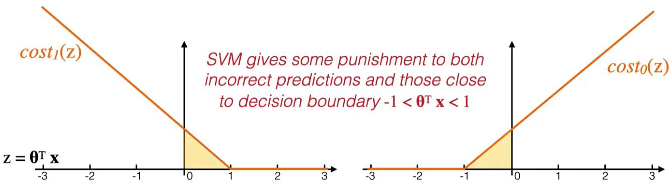
\includegraphics[width=0.9\textwidth]{images/SVM2.png} \\ \\
    \end{tabular}
\end{center}
The Loss Function of SVM is called \textbf{Hinge Loss} and is defined as follows:
\begin{equation} \tag{Hinge Loss}
    \text{cost}(h_{\theta}(x_i),y_i) =
    \begin{cases}
        max(0, 1 - \theta^Tx_i) & \text{if } y_i = 1 \\
        max(0, 1 + \theta^Tx_i) & \text{if } y_i = 0
    \end{cases}
\end{equation}
With this loss function an equidistant margin will be selected from the various examples. \\
We can rewrite the optimization objective as follows:
\begin{equation} \tag*{}
    \min \frac{1}{2} \sum^n_{j=1} \theta^2_j = \frac{1}{2} \|\theta\|^2
    \quad\Rightarrow\quad
    \begin{cases}
        \theta^Tx_i \geq 1 & \text{if } y_i = 1 \\
        \theta^Tx_i \leq -1 & \text{if } y_i = 0
    \end{cases}
\end{equation}
In case we were in two dimensions:
\begin{center}
    \begin{tabular}{c}
        \\ 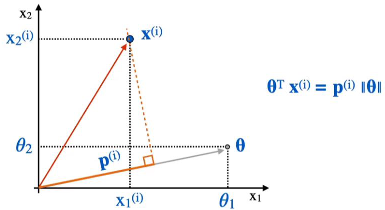
\includegraphics[width=0.5\textwidth]{images/SVM3.png} \\ \\
    \end{tabular}
\end{center}
$p_i$ is the projection of $x_i$ onto $\theta$, so $\theta^Tx_i = p_i\|\theta\|$. \\
We can rewrite the two constraints in this way:
\begin{itemize}
    \item $p_i\|\theta\| \geq 1$, if $y_i = 1$
    \item $p_i\|\theta\| \leq -1$, if $y_i = 0$
\end{itemize}
The SVM will then go to choose a decision boundary that maximizes $p_i$ since the only way to minimize the objective function is by decreasing $\theta$.

\newpage
\subsection{Margin Extension}
In case there are outliers among the examples it is necessary to introduce a way to ignore this error noise.  We can introduce into the model a variable $\xi_i$ called the \textbf{slack variable}:
\begin{equation} \tag*{}
    \min \frac{1}{2} \|\theta\|^2 + \alpha \sum^m_{i=1} \xi_i
\end{equation}
\begin{equation} \tag*{}
    \xi_i \geq 0, \forall i:y_i(p_i\|\theta\|) \geq 1 - \xi_i
\end{equation}
Extending the soft margin leads to the definition of hinge loss:
\begin{equation} \tag*{}
    l(h_\theta(x_i),y_i) = \max (0,i - y_i(\theta^Tx_i))
\end{equation}
The Hinge Loss is a convex function and can be optimized by gradient descent.

\subsection{Kernel Trick}
For classification of nonlinear data with SVM, a practice called \textbf{Kernel Trick} is used. The Kernel Trick projects the data into a new space via a function called kernel. Starting from a particular space $\mathbb{R}_n$, impose the same constraints in a higher dimensional space $\mathbb{R}_m$. The kernel function is a function $\phi:\mathbb{R}_n \rightarrow \mathbb{R}_m$ that maps vectors in $\mathbb{R}_n$ to a space $\mathbb{R}_m$.
\begin{equation}
    k(x,y) = \phi(x)^T \phi(y)
\end{equation}

\newpage